\chapter{Elliptic PDE's}
The \addtoindex{Poisson equation} is
\[ -\nabla^2U(x,y)=f(x,y), \ \ \ (x,y) \in \Omega=(0,1)\times (0,1) \]
with boundary conditions
\[u(x,y) = g(x,y), \ \ \  (x,y)\in\delta\Omega-boundary \]
\section{The five point scheme}
First we put a grid on out domain the unit square $\bar{\Omega}=[0,1]\times[0,1]=\Omega \bigcup \partial\Omega$. We will only consider a uniform grid.
\[ \triangle = \{(x_i,y_j)\in [0,1]\times[0,1]:x_i=ih,y_j=jh \}.\]
The interior nodes are
\[ \Omega_h= \{(x_i,y_j)\in \triangle:1\leq i,j\leq N-1 \}.\]
The boundary nodes are
\[ \partial\Omega_h= \{(x_0,y_j),(x_{N},y_j),(x_{i},y_0),(x_{i},y_N)
:1\leq i,j\leq N-1 \}\]
Our equations is discretised using central differencing
\begin{eqnarray*}
-(\delta_x^2w_{ij}+\delta_y^2w_{ij})&=&f_{ij} \ \ (x_i,y_j) \in \Omega_h \\
W_{ij}&=&g_{ij} \ \ (x_i,y_j) \in \partial\Omega_h 
\end{eqnarray*}
Using the central differencing we have
\[\delta_x^2=\frac{1}{h^2}(w_{i+1j}-2w_{ij}+w_{i-1j}), \]
and
\[\delta_y^2=\frac{1}{h^2}(w_{ij+1}-2w_{ij}+w_{ij-1}). \]
There for the difference equation looks like
\[-(w_{i-1j}+w_{ij-1}-4w_{ij}+w_{ij+1}+w_{i+1j})=h^2f_{ij}. \]

\begin{figure}[H]
  \caption{Graphical representation of the difference equation stencil}
  \centering
    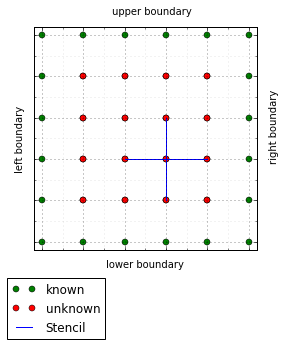
\includegraphics[width=0.5\textwidth]{PoissonEqn/Stencil}
\end{figure}
Unlike the Parabolic equation we cannot solve an Elliptic equation by holding one
variable constant and then stepping on we must solve all points at the same time.\\
We need to look at the matrix of the system of equations for the parabolic case we dealt with $(N-1)$ equations at a time, for the Hyperbolic case we must deal
with $(N-1)\times(N-1)$ equations.\\
The matrix has the following block tridiagonal structure
\begin{eqnarray*}
\left(\begin{array}{ccccccc}
T&I&0&0&.&.&.\\
I&T&I&0&0&.&.\\
0&.&.&.&0&.&.\\
.&.&.&.&.&.&.\\
.&.&.&0&I&T&I\\
.&.&.&.&0&I&T\\
\end{array}\right)
\left(\begin{array}{c}
\mathbf{w}_1\\
\mathbf{w}_2\\
.\\
.\\
\mathbf{w}_{N-2}\\
\mathbf{w}_{N-1}\\
\end{array}\right)
=-h^2
\left(\begin{array}{c}
\mathbf{r}_1\\
\mathbf{r}_2\\
.\\
.\\
\mathbf{r}_{N-2}\\
\mathbf{r}_{N-1}\\
\end{array}\right)
\end{eqnarray*}
Where $I$ denotes an $N-1 \times N-1$ identity matrix and $T$ is
\[ T=\left(\begin{array}{ccccccc}
-4&1&0&0&.&.&.\\
1&-4&1&0&0&.&.\\
0&.&.&.&0&.&.\\
.&.&.&.&.&.&.\\
.&.&.&0&1&-4&1\\
.&.&.&.&0&1&-4\\
\end{array}\right).
\]
$\mathbf{w}_j$ represents the vector of approximations
\[\mathbf{w}_j=\left(\begin{array}{c}
w_{1j}\\
w_{2j}\\
.\\
.\\
w_{N-2j}\\
w_{N-1j}\\
\end{array}\right)
\]
and $\mathbf{r}_j=\mathbf{b}_j-\mathbf{f}_j$, where $\mathbf{b}$ is the vector of 
boundary conditions 
\[\mathbf{b}_j =-\left(\begin{array}{c}
g_{0j}\\
0\\
.\\
.\\
0\\
g_{Nj}\\
\end{array}\right)
\]
for $j=2,..,N-2$, for j=1 and j=N-1 we have
\[
\mathbf{b}_1 =-\left(\begin{array}{c}
g_{01}+g_{10}\\
g_{20}\\
.\\
.\\
g_{N-20}\\
g_{N-10}+g_{1N}\\
\end{array}\right)
\mathbf{b}_{N-1} =-\left(\begin{array}{c}
g_{1N}+g_{0N-1}\\
g_{2N}\\
.\\
.\\
g_{N-2N}\\
g_{N-1N}+g_{NN-1}\\
\end{array}\right)
\]
and 
\[\mathbf{f}_j =-\left(\begin{array}{c}
f_{1j}\\
f_{2j}\\
.\\
.\\
f_{N-2j}\\
f_{N-1j}\\
\end{array}\right)
\]

\begin{figure}[H]
  \caption{Graphical representation of the large matrix}
  \centering
    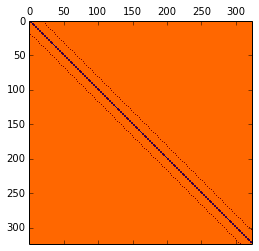
\includegraphics[width=0.5\textwidth]{PoissonEqn/large_matrix}
\end{figure}

The matrix has a unique solution. For sparse matrices of this form an iterative method is used as it would be to computationally expensive to compute the inverse.
\section{Specific Examples}
\subsection{Example 1:Homogeneous equation with non-zero boundary}
\[ \frac{\partial^2 u}{\partial x^2}+\frac{\partial^2 u}{\partial x^2}=0, \ \ \ (x,y) \in \Omega=(0,1)\times (0,1), \]
with boundary conditions:\\
Lower boundary
\[u(x,0) = \sin(2\pi x), \]
Upper boundary
\[u(x,1) = \sin(2\pi x),  \]
Left boundary
\[u(0,y) = 2*\sin(2\pi y), \]
Right boundary
\[u(1,y) =  2*\sin(2\pi y). \]
There for the difference equation looks like
\[-(w_{i-1j}+w_{ij-1}-4w_{ij}+w_{ij+1}+w_{i+1j})=0. \]

Let $N=5$

Step-size
\[h=\frac{1}{5-1}=\frac{1}{4}\]
\[\begin{array}{l|rcl}
i=1,j=1&w_{0,1}+w_{1,0}-4w_{1,1}+w_{1,2}+w_{2,1}&=&\frac{1}{4}^20\\
i=2,j=1&w_{1,1}+w_{2,0}-4w_{2,1}+w_{2,2}+w_{3,1}&=&\frac{1}{4}^20\\
i=3,j=1&w_{2,1}+w_{3,0}-4w_{3,1}+w_{3,2}+w_{4,1}&=&\frac{1}{4}^20\\
j=2\\
i=1,j=2&w_{0,2}+w_{1,1}-4w_{1,2}+w_{1,3}+w_{2,2}&=&\frac{1}{4}^20\\
i=2,j=2&w_{1,2}+w_{2,1}-4w_{2,2}+w_{2,3}+w_{3,2}&=&\frac{1}{4}^20\\
i=3,j=2&w_{2,2}+w_{3,1}-4w_{3,2}+w_{3,3}+w_{4,2}&=&\frac{1}{4}^20\\
j=3\\
i=1,j=3&w_{0,3}+w_{1,2}-4w_{1,3}+w_{1,4}+w_{2,3}&=&\frac{1}{4}^20\\
i=2,j=3&w_{1,3}+w_{2,2}-4w_{2,3}+w_{2,4}+w_{3,3}&=&\frac{1}{4}^20\\
i=3,j=3&w_{2,3}+w_{3,2}-4w_{3,3}+w_{3,4}+w_{4,3}&=&\frac{1}{4}^20\\
\end{array}
\]	

Re-arranging

\[\begin{array}{l|rcl}
i=1,j=1&-4w_{1,1}+w_{1,2}+w_{2,1}&=&\frac{1}{4}^20-w_{0,1}-w_{1,0}\\
i=2,j=1&w_{1,1}-4w_{2,1}+w_{2,2}+w_{3,1}&=&\frac{1}{4}^20-w_{2,0}\\
i=3,j=1&w_{2,1}-4w_{3,1}+w_{3,2}&=&\frac{1}{4}^20-w_{4,1}-w_{3,0}\\
j=2\\
i=1,j=2&w_{1,1}-4w_{1,2}+w_{1,3}+w_{2,2}&=&\frac{1}{4}^20-w_{0,2}\\
i=2,j=2&w_{1,2}+w_{2,1}-4w_{2,2}+w_{2,3}+w_{3,2}&=&\frac{1}{4}^20\\
i=3,j=2&w_{2,2}+w_{3,1}-4w_{3,2}+w_{3,3}&=&\frac{1}{4}^20-w_{4,2}\\
j=3\\
i=1,j=3&w_{1,2}-4w_{1,3}+w_{2,3}&=&\frac{1}{4}^20-w_{0,3}-w_{1,4}\\
i=2,j=3&w_{1,3}+w_{2,2}-4w_{2,3}+w_{3,3}&=&\frac{1}{4}^20-w_{2,4}\\
i=3,j=3&w_{2,3}+w_{3,2}-4w_{3,3}&=&\frac{1}{4}^20-w_{4,3}-w_{3,4}\\
\end{array}
\]	
Boundary Conditions
\[
\begin{array}{lcl}
\textbf{Left boundary}&\ \ \ & \textbf{Right boundary}\\ 
x_0=0&\ \ \ & x_4=1\\ 
u(0,y)=2\sin(2\pi y)&\ \ \ & u(1,y)=2\sin(2\pi y)\\

w_{0,0}=0 &\ \ \ & w_{4,0}=0\\ 
w_{0,1}=2\sin(2\pi y_1) =2 & \ \ \ & w_{4,1}=2\sin(2\pi y_1) =2\\

w_{0,2}=2\sin(2\pi y_2) =0 & \ \ \ & w_{4,2}=2\sin(2\pi y_2) =0\\

w_{0,3}=2\sin(2\pi y_3) =-2 & \ \ \ & w_{4,3}=2\sin(2\pi y_3) =-2\\

w_{0,4}=2\sin(2\pi y_4) =0 & \ \ \ & w_{4,4}=2\sin(2\pi y_4) =0\\

\end{array}
\]
\[
\begin{array}{lcl}
\textbf{Lower boundary}&\ \ \ & \textbf{Upper boundary}\\ 
 y_0=0&\ \ \ & y_4=1 \\
 u(x,0)=\sin(2\pi x)&\ \ \ & u(x,1)=\sin(2\pi x) \\

 w_{0,0}=0 & \ \ \ & w_{0,4}=0\\ 

w_{1,0}=\sin(2\pi x_1) =1  & \ \ \ & w_{1,4}=\sin(2\pi x_1) =1 \\


w_{2,0}=\sin(2\pi x_2) =0  & \ \ \ & w_{2,4}=\sin(2\pi x_2) =0 \\


w_{3,0}=\sin(2\pi x_3) =-1  & \ \ \ & w_{3,4}=\sin(2\pi x_3) =-1 \\


w_{4,0}=\sin(2\pi x_4) =0  & \ \ \ & w_{4,4}=\sin(2\pi x_4) =0 \\

\end{array}
\]

In $9\times 9$ Matrix form
\[\left(\begin{array}{ccccccccc}
-4& 1 & 0 &1 &0 &0 &0 &0 &0\\
1&-4& 1 & 0 &1 &0 &0 &0 &0 \\
0 &1&-4&  0&0 &1 &0 &0 &0 \\
1 &0 &0 &-4& 1 & 0 &1 &0 &0\\
0 & 1 &0 &1&-4& 1 &0 &1 &0  \\
0 &0 &1 &0 &1&-4&0&  0 &1  \\
0&0&0&1 &0 &0 &-4& 1 & 0\\
0&0&0&0 & 1 &0 &1&-4& 1   \\
0&0&0&0 &0 &1 &0 &1&-4
\end{array}\right)
\left(\begin{array}{c}
w_{1,1}\\
w_{2,1}\\
w_{3,1}\\
w_{1,2}\\
w_{2,2}\\
w_{3,2}\\
w_{1,3}\\
w_{2,3}\\
w_{3,3}
\end{array}\right)=
\left(\begin{array}{c}
-w_{1,0}\\
-w_{2,0}\\
-w_{3,0}\\
0\\
0\\
0\\
-w_{1,4}\\
-w_{2,4}\\
-w_{3,4}
\end{array}\right)
+\left(\begin{array}{c}
-w_{0,1}\\
0\\
-w_{4,1}\\
-w_{0,2}\\
0\\
-w_{4,2}\\
-w_{0,3}\\
0\\
-w_{4,3}
\end{array}\right)
\]	
\begin{figure}[H]
  \caption{Graphical representation of the matrix}
  \centering
    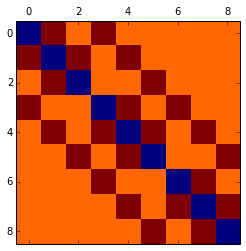
\includegraphics[width=0.5\textwidth]{PoissonEqn/matrix}
\end{figure}

In $9\times 9$ Matrix with specific values
\[\left(\begin{array}{ccccccccc}
-4& 1 & 0 &1 &0 &0 &0 &0 &0\\
1&-4& 1 & 0 &1 &0 &0 &0 &0 \\
0 &1&-4&  0&0 &1 &0 &0 &0 \\
1 &0 &0 &-4& 1 & 0 &1 &0 &0\\
0 & 1 &0 &1&-4& 1 &0 &1 &0  \\
0 &0 &1 &0 &1&-4&0&  0 &1  \\
0&0&0&1 &0 &0 &-4& 1 & 0\\
0&0&0&0 & 1 &0 &1&-4& 1   \\
0&0&0&0 &0 &1 &0 &1&-4
\end{array}\right)
\left(\begin{array}{c}
w_{1,1}\\
w_{2,1}\\
w_{3,1}\\
w_{1,2}\\
w_{2,2}\\
w_{3,2}\\
w_{1,3}\\
w_{2,3}\\
w_{3,3}
\end{array}\right)=
\left(\begin{array}{c}
-1\\
0\\
1\\
0\\
0\\
0\\
-1\\
0\\
1
\end{array}\right)
+\left(\begin{array}{c}
-2\\
0\\
-2\\
0\\
0\\
0\\
2\\
0\\
2
\end{array}\right)
\]	

\begin{figure}[H]
  \caption{Numerical solution of the homogeneous differential equation }
  \centering
    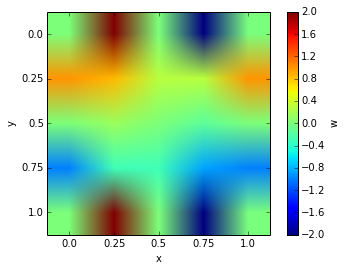
\includegraphics{PoissonEqn/solution_homogeneous}
\end{figure}

\subsection{Example 2: non-homogeneous equation with zero boundary}
\[ \frac{\partial^2 u}{\partial x^2}+\frac{\partial^2 u}{\partial x^2}=x^2+y^2 \ \ \ (x,y) \in \Omega=(0,1)\times (0,1) \]
with boundary conditions:
Left boundary:
\[u(x,0) =0 \]
Right boundary:
\[u(x,1) = 0  \]
Lower boundary:
\[u(0,y) = 0 \]
Upper boundary:
\[u(1,y) =  0 \]
There for the difference equation looks like
\[-(w_{i-1j}+w_{ij-1}-4w_{ij}+w_{ij+1}+w_{i+1j})=h^2(x_i^2+y_j^2). \]

Let $N=5$

Step-size
\[h=\frac{1}{5-1}=\frac{1}{4}\]
\[\begin{array}{l|rcl}
i=1,j=1&w_{0,1}+w_{1,0}-4w_{1,1}+w_{1,2}+w_{2,1}&=&\frac{1}{4}^2(x_1^2+y_1^2)\\
i=2,j=1&w_{1,1}+w_{2,0}-4w_{2,1}+w_{2,2}+w_{3,1}&=&\frac{1}{4}^2(x_2^2+y_1^2)\\
i=3,j=1&w_{2,1}+w_{3,0}-4w_{3,1}+w_{3,2}+w_{4,1}&=&\frac{1}{4}^2(x_3^2+y_1^2)\\
j=2\\
i=1,j=2&w_{0,2}+w_{1,1}-4w_{1,2}+w_{1,3}+w_{2,2}&=&\frac{1}{4}^2(x_1^2+y_2^2)\\
i=2,j=2&w_{1,2}+w_{2,1}-4w_{2,2}+w_{2,3}+w_{3,2}&=&\frac{1}{4}^2(x_2^2+y_2^2)\\
i=3,j=2&w_{2,2}+w_{3,1}-4w_{3,2}+w_{3,3}+w_{4,2}&=&\frac{1}{4}^2(x_3^2+y_2^2)\\
j=3\\
i=1,j=3&w_{0,3}+w_{1,2}-4w_{1,3}+w_{1,4}+w_{2,3}&=&\frac{1}{4}^2(x_1^2+y_3^2)\\
i=2,j=3&w_{1,3}+w_{2,2}-4w_{2,3}+w_{2,4}+w_{3,3}&=&\frac{1}{4}^2(x_2^2+y_3^2)\\
i=3,j=3&w_{2,3}+w_{3,2}-4w_{3,3}+w_{3,4}+w_{4,3}&=&\frac{1}{4}^2(x_3^2+y_3^2)\\
\end{array}
\]	

Re-arranging

\[\begin{array}{l|rcl}
i=1,j=1&-4w_{1,1}+w_{1,2}+w_{2,1}&=&\frac{1}{4}^2(x_1^2+y_1^2)-w_{0,1}-w_{1,0}\\
i=2,j=1&w_{1,1}-4w_{2,1}+w_{2,2}+w_{3,1}&=&\frac{1}{4}^2(x_2^2+y_1^2)-w_{2,0}\\
i=3,j=1&w_{2,1}-4w_{3,1}+w_{3,2}&=&\frac{1}{4}^2(x_3^2+y_1^2)-w_{4,1}-w_{3,0}\\
j=2\\
i=1,j=2&w_{1,1}-4w_{1,2}+w_{1,3}+w_{2,2}&=&\frac{1}{4}^2(x_1^2+y_2^2)-w_{0,2}\\
i=2,j=2&w_{1,2}+w_{2,1}-4w_{2,2}+w_{2,3}+w_{3,2}&=&\frac{1}{4}^2(x_2^2+y_2^2)\\
i=3,j=2&w_{2,2}+w_{3,1}-4w_{3,2}+w_{3,3}&=&\frac{1}{4}^2(x_3^2+y_2^2)-w_{4,2}\\
j=3\\
i=1,j=3&w_{1,2}-4w_{1,3}+w_{2,3}&=&\frac{1}{4}^2(x_1^2+y_3^2)-w_{0,3}-w_{1,4}\\
i=2,j=3&w_{1,3}+w_{2,2}-4w_{2,3}+w_{3,3}&=&\frac{1}{4}^2(x_2^2+y_3^2)-w_{2,4}\\
i=3,j=3&w_{2,3}+w_{3,2}-4w_{3,3}&=&\frac{1}{4}^2(x_3^2+y_3^2)-w_{4,3}-w_{3,4}\\
\end{array}
\]	
Boundary Conditions
\[
\begin{array}{lcl}
\textbf{Left Boundary}&\ \ \ & \textbf{Right Boundary} \\
x_0=0&\ \ \ & x_4=1\\
u(0,y)=0&\ \ \ & u(1,y)=0\\
w_{0,0}=0 &\ \ \ & w_{4,0}=0 \\ 
w_{0,1}=0& \ \ \ & w_{4,1}=0 \\
w_{0,2}=0 & \ \ \ & w_{4,2}=0  \\
w_{0,3}=0& \ \ \ & w_{4,3}=0  \\
w_{0,4}=0 & \ \ \ & w_{4,4}=0  \\

\end{array}
\]
\[
\begin{array}{lcl}
\textbf{Left Boundary}&\ \ \ & \textbf{Right Boundary} \\
y_0=0&\ \ \ & y_4=1 \\
u(x,0)=0&\ \ \ & u(x,1)=0 \\

w_{0,0}=0 & \ \ \ & w_{0,4}=0\\ 
w_{1,0}=0  & \ \ \ & w_{1,4}=0 \\
w_{2,0}=0  & \ \ \ & w_{2,4}=0 \\
w_{3,0}=0  & \ \ \ & w_{3,4}=0 \\
w_{4,0}=0  & \ \ \ & w_{4,4}=0 \\

\end{array}
\]

In $9\times 9$ Matrix form
\[\left(\begin{array}{ccccccccc}
-4& 1 & 0 &1 &0 &0 &0 &0 &0\\
1&-4& 1 & 0 &1 &0 &0 &0 &0 \\
0 &1&-4&  0&0 &1 &0 &0 &0 \\
1 &0 &0 &-4& 1 & 0 &1 &0 &0\\
0 & 1 &0 &1&-4& 1 &0 &1 &0  \\
0 &0 &1 &0 &1&-4&0&  0 &1  \\
0&0&0&1 &0 &0 &-4& 1 & 0\\
0&0&0&0 & 1 &0 &1&-4& 1   \\
0&0&0&0 &0 &1 &0 &1&-4
\end{array}\right)
\left(\begin{array}{c}
w_{1,1}\\
w_{2,1}\\
w_{3,1}\\
w_{1,2}\\
w_{2,2}\\
w_{3,2}\\
w_{1,3}\\
w_{2,3}\\
w_{3,3}
\end{array}\right)=
h^2\left(\begin{array}{c}
(x_1^2+y_1^2)\\
(x_2^2+y_1^2)\\
(x_3^2+y_1^2)\\
(x_1^2+y_2^2)\\
(x_2^2+y_2^2)\\
(x_3^2+y_2^2)\\
(x_1^2+y_3^2)\\
(x_2^2+y_3^2)\\
(x_3^2+y_3^2)
\end{array}\right)
\]	

In $9\times 9$ Matrix form
\[\left(\begin{array}{ccccccccc}
-4& 1 & 0 &1 &0 &0 &0 &0 &0\\
1&-4& 1 & 0 &1 &0 &0 &0 &0 \\
0 &1&-4&  0&0 &1 &0 &0 &0 \\
1 &0 &0 &-4& 1 & 0 &1 &0 &0\\
0 & 1 &0 &1&-4& 1 &0 &1 &0  \\
0 &0 &1 &0 &1&-4&0&  0 &1  \\
0&0&0&1 &0 &0 &-4& 1 & 0\\
0&0&0&0 & 1 &0 &1&-4& 1   \\
0&0&0&0 &0 &1 &0 &1&-4
\end{array}\right)
\left(\begin{array}{c}
w_{1,1}\\
w_{2,1}\\
w_{3,1}\\
w_{1,2}\\
w_{2,2}\\
w_{3,2}\\
w_{1,3}\\
w_{2,3}\\
w_{3,3}
\end{array}\right)=
\left(\begin{array}{c}
0.0078125\\
0.01953125\\
0.0390625 \\
 0.01953125\\
 0.0312\\
0.05078125\\
0.0390625\\
0.05078125\\
0.0703125
\end{array}\right)
\]	
\begin{figure}[H]
  \caption{Numerical solution of the differential equation with 0 boundary conditions }
  \centering
    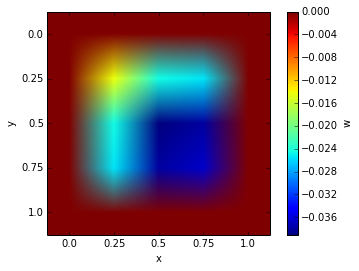
\includegraphics{PoissonEqn/solution_zero_boundary}
\end{figure}

\subsection{Example 3: Inhomogeneous equation with non-zero boundary}
\[ \frac{\partial^2 u}{\partial x^2}+\frac{\partial^2 u}{\partial x^2}=xy, \ \ \ (x,y) \in \Omega=(0,1)\times (0,1), \]
with boundary conditions\\
Right Boundary
\[u(x,0) =-x^2+x \]
Left Boundary
\[u(x,1) = x^2-x  \]
Lower Boundary
\[u(0,y) = -y^2+y \]
Upper Boundary
\[u(1,y) =  -y^2+y \]
There for the difference equation looks like
\[-(w_{i-1j}+w_{ij-1}-4w_{ij}+w_{ij+1}+w_{i+1j})=h^2(x_iy_j). \]

Let $N=5$

Step-size
\[h=\frac{1}{5-1}=\frac{1}{4}\]
\[\begin{array}{l|rcl}
i=1,j=1&w_{0,1}+w_{1,0}-4w_{1,1}+w_{1,2}+w_{2,1}&=&\frac{1}{4}^2(x_1y_1)\\
i=2,j=1&w_{1,1}+w_{2,0}-4w_{2,1}+w_{2,2}+w_{3,1}&=&\frac{1}{4}^2(x_2y_1)\\
i=3,j=1&w_{2,1}+w_{3,0}-4w_{3,1}+w_{3,2}+w_{4,1}&=&\frac{1}{4}^2(x_3y_1)\\
j=2\\
i=1,j=2&w_{0,2}+w_{1,1}-4w_{1,2}+w_{1,3}+w_{2,2}&=&\frac{1}{4}^2(x_1y_2)\\
i=2,j=2&w_{1,2}+w_{2,1}-4w_{2,2}+w_{2,3}+w_{3,2}&=&\frac{1}{4}^2(x_2y_2)\\
i=3,j=2&w_{2,2}+w_{3,1}-4w_{3,2}+w_{3,3}+w_{4,2}&=&\frac{1}{4}^2(x_3y_2)\\
j=3\\
i=1,j=3&w_{0,3}+w_{1,2}-4w_{1,3}+w_{1,4}+w_{2,3}&=&\frac{1}{4}^2(x_1y_3)\\
i=2,j=3&w_{1,3}+w_{2,2}-4w_{2,3}+w_{2,4}+w_{3,3}&=&\frac{1}{4}^2(x_2y_3)\\
i=3,j=3&w_{2,3}+w_{3,2}-4w_{3,3}+w_{3,4}+w_{4,3}&=&\frac{1}{4}^2(x_3y_3)\\
\end{array}
\]	

Re-arranging

\[\begin{array}{l|rcl}
i=1,j=1&-4w_{1,1}+w_{1,2}+w_{2,1}&=&\frac{1}{4}^2(x_1y_1)-w_{0,1}-w_{1,0}\\
i=2,j=1&w_{1,1}-4w_{2,1}+w_{2,2}+w_{3,1}&=&\frac{1}{4}^2(x_2y_1)-w_{2,0}\\
i=3,j=1&w_{2,1}-4w_{3,1}+w_{3,2}&=&\frac{1}{4}^2(x_3y_1)-w_{4,1}-w_{3,0}\\
j=2\\
i=1,j=2&w_{1,1}-4w_{1,2}+w_{1,3}+w_{2,2}&=&\frac{1}{4}^2(x_1y_2)-w_{0,2}\\
i=2,j=2&w_{1,2}+w_{2,1}-4w_{2,2}+w_{2,3}+w_{3,2}&=&\frac{1}{4}^2(x_2y_2)\\
i=3,j=2&w_{2,2}+w_{3,1}-4w_{3,2}+w_{3,3}&=&\frac{1}{4}^2(x_3y_2)-w_{4,2}\\
j=3\\
i=1,j=3&w_{1,2}-4w_{1,3}+w_{2,3}&=&\frac{1}{4}^2(x_1y_3)-w_{0,3}-w_{1,4}\\
i=2,j=3&w_{1,3}+w_{2,2}-4w_{2,3}+w_{3,3}&=&\frac{1}{4}^2(x_2y_3)-w_{2,4}\\
i=3,j=3&w_{2,3}+w_{3,2}-4w_{3,3}&=&\frac{1}{4}^2(x_3y_3)-w_{4,3}-w_{3,4}\\
\end{array}
\]	

Boundary Conditions
\[
\begin{array}{lcl}
\textbf{Left boundary}&\ \ \ & \textbf{Right boundary}\\ 
x_0=0&\ \ \ & x_4=1\\ 
u(0,y)=-y^2+y&\ \ \ & u(1,y)=-y^2+y\\

w_{0,0}=0 &\ \ \ & w_{4,0}=0\\ 
w_{0,1}=-y^2_1+y_1 =\frac{3}{16} & \ \ \ & w_{4,1}=-y^2_1+y_1 =\frac{1}{16}\\

w_{0,2}=-y^2_2+y_2 =\frac{1}{4} & \ \ \ & w_{4,2}=-y^2_2+y_2 =\frac{1}{4}\\

w_{0,3}=-y^2_3+y_3 =\frac{3}{16} & \ \ \ & w_{4,3}=-y^2_3+y_3 =\frac{3}{16}\\

w_{0,4}=-y^2_4+y_4 =0 & \ \ \ & w_{4,4}=-y^2_4+y_4 =0\\

\end{array}
\]
\[
\begin{array}{lcl}
\textbf{Lower boundary}&\ \ \ & \textbf{Upper boundary}\\ 
 y_0=0&\ \ \ & y_4=1 \\
 u(x,0)=-x^2+x&\ \ \ & u(x,1)=x^2-x \\

 w_{0,0}=0 & \ \ \ & w_{0,4}=0\\ 

w_{1,0}=-x^2_1+x_1 =\frac{3}{16}  & \ \ \ & w_{1,4}=x^2_1-x_1 =-\frac{3}{16} \\


w_{2,0}=-x^2_2+x_2 =\frac{1}{4}  & \ \ \ & w_{2,4}=x^2_2-x_2 =-\frac{1}{4} \\


w_{3,0}=-x^2_3+x_3 =\frac{3}{16}  & \ \ \ & w_{3,4}=x^2_3-x_3 =-\frac{3}{16} \\


w_{4,0}=0  & \ \ \ & w_{4,4}=0 \\

\end{array}
\]

In $9\times 9$ Matrix form
\[\left(\begin{array}{ccccccccc}
-4& 1 & 0 &1 &0 &0 &0 &0 &0\\
1&-4& 1 & 0 &1 &0 &0 &0 &0 \\
0 &1&-4&  0&0 &1 &0 &0 &0 \\
1 &0 &0 &-4& 1 & 0 &1 &0 &0\\
0 & 1 &0 &1&-4& 1 &0 &1 &0  \\
0 &0 &1 &0 &1&-4&0&  0 &1  \\
0&0&0&1 &0 &0 &-4& 1 & 0\\
0&0&0&0 & 1 &0 &1&-4& 1   \\
0&0&0&0 &0 &1 &0 &1&-4
\end{array}\right)
\left(\begin{array}{c}
w_{1,1}\\
w_{2,1}\\
w_{3,1}\\
w_{1,2}\\
w_{2,2}\\
w_{3,2}\\
w_{1,3}\\
w_{2,3}\\
w_{3,3}
\end{array}\right)=\]
\[
h^2\left(\begin{array}{c}
(x_1y_1)\\
(x_2y_1)\\
(x_3y_1)\\
(x_1y_2)\\
(x_2y_2)\\
(x_3y_2)\\
(x_1y_3)\\
(x_2y_3)\\
(x_3y_3)
\end{array}\right)+
\left(\begin{array}{c}
-w_{1,0}\\
-w_{2,0}\\
-w_{3,0}\\
0\\
0\\
0\\
-w_{1,4}\\
-w_{2,4}\\
-w_{3,4}
\end{array}\right)
+\left(\begin{array}{c}
-w_{0,1}\\
0\\
-w_{4,1}\\
-w_{0,2}\\
0\\
-w_{4,2}\\
-w_{0,3}\\
0\\
-w_{4,3}
\end{array}\right)
\]	

In $9\times 9$ Matrix form
\[\left(\begin{array}{ccccccccc}
-4& 1 & 0 &1 &0 &0 &0 &0 &0\\
1&-4& 1 & 0 &1 &0 &0 &0 &0 \\
0 &1&-4&  0&0 &1 &0 &0 &0 \\
1 &0 &0 &-4& 1 & 0 &1 &0 &0\\
0 & 1 &0 &1&-4& 1 &0 &1 &0  \\
0 &0 &1 &0 &1&-4&0&  0 &1  \\
0&0&0&1 &0 &0 &-4& 1 & 0\\
0&0&0&0 & 1 &0 &1&-4& 1   \\
0&0&0&0 &0 &1 &0 &1&-4
\end{array}\right)
\left(\begin{array}{c}
w_{1,1}\\
w_{2,1}\\
w_{3,1}\\
w_{1,2}\\
w_{2,2}\\
w_{3,2}\\
w_{1,3}\\
w_{2,3}\\
w_{3,3}
\end{array}\right)=\]
\[
\left(\frac{1}{4}\right)^2\left(\begin{array}{c}
0.0625\\
0.125\\
0.1875 \\
0.125\\
 0.25\\
0.375\\
0.1875\\
0.375\\
0.5626
\end{array}\right)
+\left(\begin{array}{c}
-\frac{3}{16}\\
-\frac{1}{4}\\
-\frac{3}{16}\\
0\\
0\\
0\\
\frac{3}{16}\\
\frac{1}{4}\\
\frac{3}{16}
\end{array}\right)
+\left(\begin{array}{c}
-\frac{3}{16}\\
0\\
-\frac{3}{16}\\
-\frac{1}{4}\\
0\\
-\frac{1}{4}\\
-\frac{3}{16}\\
0\\
-\frac{3}{16}
\end{array}\right)
\]	

\begin{figure}[H]
  \caption{Numerical solution of the differential equation with non-zero boundary conditions }
  \centering
    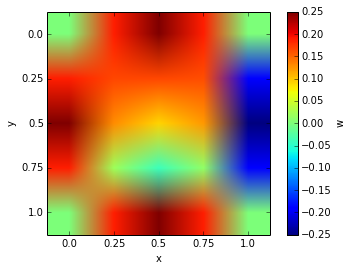
\includegraphics{PoissonEqn/Solution_full_equation}
\end{figure}

\section{Consistency and Convergence}
We now ask how well the grid function determined by the five point scheme approximates
the exact solution of the Poisson problem.
\begin{definition}
Let $L_h$ denote the finite difference approximation associated with the grid $\Omega_h$ having the mesh size $h$, to a partial differential operator $L$ defined on
a simply connected, open set $\Omega \subset R^2$. For a given function $\varphi\in C^{\infty}(\Omega)$,
the truncation error of $L_h$ is
\[\tau_{h}(\mathbf{x})=(L-L_h)\varphi(x) \]
The approximation $L_h$ is consistent with $L$ if
\[ \lim_{h\rightarrow 0}\tau_h(x)=0,\]
for all $\mathbf{x} \in D$ and all $\varphi \in C^{\infty}(\Omega)$. The approximation is consistent to order $p$ if $\tau_h(\mathbf{x})=O(h^p)$.
$\circ$
\end{definition}
While we have seen this definition a few times it is always interesting how the
terms are denoted and expressed but the ideas are always the same.
\begin{proposition}
The five-point difference analog $-\nabla^2_h$ is consistent to order 2 with $-\nabla^2$.
\end{proposition}
\begin{proof}
Pick $\varphi \in C^{\infty}(D)$, and let $(x,y) \in \Omega$ be a point such that $(x\pm h, y),(x,y \pm h) \in \Omega\bigcup \partial\Omega$.  By the Taylor Theorem
\begin{eqnarray*}
\varphi(x\pm h,y)&=&\varphi(x,y) \pm h \frac{\partial \varphi}{\partial x}(x,y)+\frac{h^2}{2!}\frac{\partial^2 \varphi}{\partial x^2}(x,y) \pm\frac{h^3}{3!}\frac{\partial^3 \varphi}{\partial x^3}(x,y)+\frac{h^4}{4!}\frac{\partial^4 \varphi}{\partial x^4}(\zeta^{\pm},y)
\end{eqnarray*}
where $\zeta^{\pm} \in (x-h,x+h)$. Adding this pair of equation together and rearranging , we get
\[\frac{1}{h^2}[\varphi(x+h,y)-2\varphi(x,y)+\varphi(x-h,y) ] -\frac{\partial^2 \varphi}{\partial x^2}(x,y)=\frac{h^2}{4!}\left[\frac{\partial^4 \varphi}{\partial x^4}(\zeta^{+},y)+
\frac{\partial^4 \varphi}{\partial x^4}(\zeta^{-},y)
 \right]
\]
By the intermediate value theorem
\[\left[\frac{\partial^4 \varphi}{\partial x^4}(\zeta^{+},y)+
\frac{\partial^4 \varphi}{\partial x^4}(\zeta^{-},y)
 \right]
=2\frac{\partial^4 \varphi}{\partial x^4}(\zeta,y),\]
for some $\zeta \in (x-h,x+h)$.  Therefore,
\[\delta_x^2(x,y)
=\frac{\partial^2 \varphi}{\partial x^2}(x,y)+\frac{h^2}{2!}\frac{\partial^4 \varphi}{\partial x^4}(\zeta,y)
\]
Similar reasoning shows that
\[\delta_y^2(x,y)
=\frac{\partial^2 \varphi}{\partial y^2}(x,y)+\frac{h^2}{2!}\frac{\partial^4 \varphi}{\partial y^4}(x,\eta)
\]
for some $\eta \in (y-h,y+h)$. We conclude that $\tau_h(x,y)=(\nabla-\nabla_h)\varphi(x,y)=O(h^2).$
$\bullet$\end{proof}
Consistency does not guarantee that the solution to the difference equations approximates the exact solution to the \addtoindex{PDE}. 
\begin{definition}
Let $L_hw(\mathbf{x}_j)=f(\mathbf{x}_j)$ be a finite difference approximation, defined on a grid mesh size h, to a \addtoindex{PDE} $LU(\mathbf{x})=f(\mathbf{x})$ on a simply
connected set $D \subset R^n$. Assume that $w(x,y)=U(x,y)$ at all points (x,y) on the boundary $\partial\Omega$.  The finite difference scheme converges (or is convergent) if
\[ \max_j|U(\mathbf{x}_j)-w(\mathbf{x}_j)| \rightarrow 0 \mbox{  as  } h \rightarrow 0.\]
$\circ$
\end{definition}
For the five point scheme there is a direct connection between consistency and convergence.  Underlying this connection is an argument based on the following principle:
\begin{theorem}
(DISCRETE MAXIMUM PRINCIPLE).
If $\nabla^2_hV_{ij}\geq 0$ for all points $(x_i,y_j) \in \Omega_h$, then
\[ \max_{(x_i,y_j)\in\Omega_h}V_{ij}\leq  \max_{(x_i,y_j)\in\partial\Omega_h}V_{ij}\]
If $\nabla^2_hV_{ij}\leq 0$ for all points $(x_i,y_j) \in \Omega_h$, then
\[ \min_{(x_i,y_j)\in\Omega_h}V_{ij}\geq  \min_{(x_i,y_j)\in\partial\Omega_h}V_{ij}\]
\end{theorem}
In other words, a grid function $V$ for which $\nabla^2_hV$ is nonnegative on $\Omega_h$ attains its maximum on the boundary $\partial\Omega_h$ of the grid.  Similarly, if $\nabla^2_hV$ is nonpositive on $\Omega_h$, then V attains its minimum on the boundary $\partial\Omega_h$.
\begin{proof}
The proof is by contradiction.  We argue for the case $\nabla_h^2V_{ij} \geq 0$, reasoning for the case $\nabla_h^2V_{ij}\leq 0$ begin similar.\\
Assume that $V$ attains its maximum value M at an interior grid point $(x_I,y_J)$ and that $\max_{(x_i,y_j)\in\partial\Omega_h}V_{ij}<M.$ The hypothesis $\nabla_{h}^2V_{ij} \geq 0$ implies that
\[ V_{IJ}\leq\frac{1}{4}(V_{I+1J}+V_{I-1J}+V_{IJ+1}+V_{IJ-1}) \]
This cannot hold unless
\[ V_{I+1J}=V_{I-1J}=V_{IJ+1}=V_{IJ-1}=M. \]
If any of the corresponding grid points $(x_{I+1},y_{L}),(x_{J-1},y_{L}),(x_{I},y_{L+1}),(x_{I},y_{L-1})$ lies in $\partial\Omega_h$, then we have reached the 
desired contradiction.\\
Otherwise, we continue arguing in this way until we conclude that $V_{I+iJ+j}=M$
for some point $(x_{I+iJ+j})\in \partial\Omega$, which again gives a contradiction.
$\bullet$\end{proof}
This leads to interesting results
\begin{proposition}
\begin{enumerate}
\item
The zero grid function (for which $U_{ij}=0$ for all $(x_i,y_j) \in \Omega_h \bigcup \partial\Omega_h$
is the only solution to the finite difference problem
\[\nabla_h^2U_{ij}=0 \mbox{ for }(x_i,y_j)\in\Omega_h,\]
\[U_{ij}=0 \mbox{ for }(x_i,y_j)\in\partial\Omega_h.\]
\item
For prescribed grid functions $f_{ij}$ and $g_{ij}$, there exists a unique solution to the problem
\[\nabla_h^2U_{ij}=f_{ij} \mbox{ for }(x_i,y_j)\in\Omega_h,\]
\[U_{ij}=g_{ij} \mbox{ for }(x_i,y_j)\in\partial\Omega_h.\]
\end{enumerate}
\end{proposition}
\begin{definition}
For any grid function $V:\Omega_h\bigcup\partial\Omega_h \rightarrow R$,
\[||V||_{\Omega} =\max_{(x_i,y_j)\in\Omega_h}|V_{ij}|, \]
\[||V||_{\partial\Omega} =\max_{(x_i,y_j)\in\partial\Omega_h}|V_{ij}|. \]
$\circ$
\end{definition}
\begin{lemma}
If the grid function $V:\Omega_h\bigcup\partial\Omega_h\rightarrow R$ satisfies the boundary condition $V_{ij}=0$ for $(x_i,y_j)\in \partial\Omega_h$, then
\[||V_||_{\Omega}\leq \frac{1}{8}||\nabla_h^2V||_{\Omega} \]
\end{lemma}
\begin{proof}
Let $\nu = ||\nabla_{h}^2V||_{\Omega}$. Clearly for all points $(x_i,y_j)\in\Omega_h$,
\begin{equation}\label{ineq 828}
-\nu \leq \nabla_{h}^2V_{ij} \leq \nu \end{equation}
Now we define $W:\Omega_h \bigcup \partial\Omega_h \rightarrow R$ by setting 
$W_{ij}=\frac{1}{4}[(x_i-\frac{1}{2})^2+(y_j-\frac{1}{2})^2]$, which is nonnegative.  Also $\nabla_h^2W_{ij}=1$ and that $||W||_{\partial\Omega}=\frac{1}{8}$.
The inequality (\ref{ineq 828}) implies that, for all points $(x_i,y_j)\in\Omega_h$,
\[\nabla_h^2(V_{ij}+\nu W_{ij})\geq 0 \]
\[\nabla_h^2(V_{ij}-\nu W_{ij})\leq 0 \]
By the discrete minimum principle and the fact that V vanishes on $\partial\Omega_h$
\[V_{ij}\leq V_{ij}+\nu W_{ij}\leq \nu||W||_{\partial\Omega} \]
\[V_{ij}\geq V_{ij}-\nu W_{ij}\geq -\nu||W||_{\partial\Omega} \]
Since $||W||_{\partial\Omega}=\frac{1}{8}$
\[||V_||_{\Omega}\leq \frac{1}{8}\nu =\frac{1}{8}||\nabla_h^2V||_{\Omega} \]
$\bullet$\end{proof}
Finally we prove that the five point scheme for the \addtoindex{Poisson equation} is convergent.
\begin{theorem}
Let $U$ be a solution to the \addtoindex{Poisson equation} and let $w$ be the grid function
that satisfies the discrete analog
\[-\nabla_h^2w_{ij}=f_{ij} \ \ \mbox{ for } (x_i,y_j)\in\Omega_h, \]
\[w_{ij}=g_{ij} \ \ \mbox{ for } (x_i,y_j)\in\partial\Omega_h. \]
Then there exists a positive constant $K$ such that
\[||U-w||_{\Omega}\leq KMh^2 \]
where
\[ M=\left\{
\left|\left|\frac{\partial^4 U}{\partial x^4} \right|\right|_{\infty},
\left|\left|\frac{\partial^4 U}{\partial x^3\partial y} \right|\right|_{\infty},
...,
\left|\left|\frac{\partial^4 U}{\partial y^4} \right|\right|_{\infty}
 \right\}
\]
\end{theorem}
The statement of the theorem assumes that $U\in C^4(\bar{\Omega})$. This assumption
holds if $f$ and $g$ are smooth enough.
\begin{proof}
Following from the proof of the Proposition we have
\[ (\nabla_h^2-\nabla^2)U_{ij}=\frac{h^2}{12}\left[ \frac{\partial^4 U}{\partial x^4}(\zeta_i,y_j)+\frac{\partial^4 U}{\partial y^4}(x_i,\eta_j) \right]\]
for some $\zeta \in (x_{i-1},x_{i+1})$ and $\eta_j\in(y_{j-1},y_{j+1})$.  Therefore,
\[ -\nabla_h^2U_{ij}=f_{ij}-\frac{h^2}{12}\left[ \frac{\partial^4 U}{\partial x^4}(\zeta_i,y_j)+\frac{\partial^4 U}{\partial y^4}(x_i,\eta_j) \right].\]
If we subtract from this the identity equation $-\nabla_h^2w_{ij}=f_{ij}$ and note
that $U-w$ vanishes on $\partial\Omega_h$, we find that
\[ \nabla_h^2(U_{ij}-w_{ij})=\frac{h^2}{12}\left[ \frac{\partial^4 U}{\partial x^4}(\zeta_i,y_j)+\frac{\partial^4 U}{\partial y^4}(x_i,\eta_j) \right].\]
It follows that
\[ ||U-w||_{\Omega}\leq\frac{1}{8}||\nabla_h^2(U-w)||_{\Omega}\leq KMh^2\]
\end{proof}